% Selection or Teaching? Value Added and Cost in Brazilian Federal Universities
% Working paper, draft v0.6 (November 2026)
\documentclass[11pt,a4paper]{article}
\usepackage{fontspec}
\setmainfont{TeX Gyre Pagella}
\usepackage[english]{babel}
\usepackage[a4paper,margin=2.6cm]{geometry}
\usepackage{setspace}
\setstretch{1.25}
\usepackage{microtype}
\usepackage{amsmath,amssymb}
\usepackage{booktabs,array,threeparttable}
\usepackage{graphicx}
\usepackage{caption}
\captionsetup{font=small,labelfont=bf}
\usepackage[round]{natbib}
\usepackage{xcolor}
\usepackage[colorlinks=true,linkcolor=black,citecolor=black,urlcolor=blue!50!black]{hyperref}
\usepackage{xurl}
\newcommand{\todo}[1]{\par\noindent\colorbox{yellow!25}{\parbox{\dimexpr\linewidth-2\fboxsep}{\small\textbf{TO DO:} #1}}\par}

\title{\textbf{Selection or Teaching?}\\[0.2em]\large Value Added and Cost in Brazilian Federal Universities}
\author{Caio A. F. Cunha\thanks{Independent researcher. ORCID: \href{https://orcid.org/0009-0008-2153-901X}{0009-0008-2153-901X}. Data, code and replication instructions: \url{https://github.com/Caioalexnes/higher-education-analysis}.}}
\date{Working paper, draft v0.6, November 2026}

\begin{document}
\maketitle

\begin{abstract}
\noindent Brazilian federal universities are tuition-free, admit students through a national exam and lead every raw indicator of higher-education quality. This paper asks how much of their advantage is selection and how much is teaching. Using course-level results of the national graduation exam (Enade) and the official value-added indicator that nets out each graduate's admission-exam score (IDD), and comparing only courses in the same assessment area, federal graduates score 12.7 points above graduates of for-profit private courses in 2023 and 11.7 points in 2022, on a 0--100 scale. Their value-added advantage is 2.6 and 2.7 points: about four fifths of the raw gap was already present at entry. The pattern holds with controls for modality, institution type, size, state and entering-cohort composition, and in every robustness check. Where federal courses face little competition for seats, the raw gap falls by about half while the value-added gap shows no clear change. The method INEP used to compute the IDD until 2021 averaged out most of each course's own effect, and the published IDD of those editions shows almost no value-added gap between federal and private courses. Recomputing the indicator with the current method from INEP's student-level data, which reproduces the published values exactly, the federal value-added advantage is positive in every edition from 2016 to 2023 and grows from about 1 point to 2.6--2.7 points, while between 71\% and 91\% of the raw gap was present at entry in every edition. Among 66 federal universities, current spending per student is not significantly associated with value added.

\medskip
\noindent\textbf{Keywords:} higher education; value added; selection; public universities; Brazil; Enade.\\
\noindent\textbf{JEL codes:} I23; I22; H52.
\end{abstract}

\newpage
%======================================================================
\section{Introduction}\label{sec:intro}
%======================================================================

In Brazil, federal universities are free of tuition, are financed entirely by the federal government and are widely regarded as the best institutions in the country. On every raw indicator of quality published by the Ministry of Education they lead the private sector, which enrols about four in five undergraduates. In the 2023 national graduation exam, 63.7\% of federal courses obtained the two highest grades of the official course score, against 10.4\% of courses offered by for-profit private institutions. Federal universities also cost more per student. The World Bank estimated spending per student in Brazilian public universities at two to five times that of private institutions \citep{worldbank2017}, and a later study that disputes this estimate still finds a difference of about one and a half times \citep{bielschowsky2022}.

A raw comparison of outcomes cannot tell whether federal universities teach more or simply admit students who are better prepared to learn. The admission exam measures what students know at the end of secondary school, and what they know reflects how much and how well they have been able to study, which also predicts how much they will learn in higher education. Admission to federal universities runs through a centralized platform (Sisu) that ranks applicants by their score in the national secondary-school exam (Enem), so the most demanded courses fill their seats with applicants from the top of the national distribution. Graduates' scores therefore mix what students brought at entry with what the institution added. This paper separates the two components with an indicator published by the national assessment agency (INEP): the IDD, which compares the scores of each course's graduates in the graduation exam (Enade) with the scores predicted by their Enem results, in a multilevel model estimated for each area \citep{inep2023idd}. Because the IDD and the raw Enade score are on the same scale, the federal advantage can be decomposed into a part that was present at entry and a part that corresponds to value added.

The paper makes four contributions. First, it measures, for the two most recent editions (2022 and 2023, which assessed different groups of areas), how much of the raw advantage of federal courses over private courses in the same area is selection and how much is value added, with confidence intervals and, for 2023, with regressions that control for modality, institution type, course size, state and the composition of the entering cohort. Second, it tests a direct implication of the selection explanation: the federal advantage should shrink where federal courses face little competition for seats. Third, it shows that the method used to compute the IDD until 2021 removed most of each course's own effect from the indicator, the more so the larger the course, and recomputes the IDD of every edition from 2016 to 2023 with both definitions from INEP's student-level microdata, reproducing the published values exactly. With a consistent definition, the federal value-added advantage is positive in every edition and grows over time; with the published values it is close to zero until 2021. Any comparison of institutions based on the published IDD of the earlier editions is affected by the same compression. Fourth, it relates value added to current spending per student across 66 federal universities.

The answer to the main question is that selection explains most of the federal advantage. Comparing courses in the same area, federal graduates score 12.7 points above for-profit private graduates in 2023, on a 0--100 scale whose within-area student standard deviation is 13.6 points, and 11.7 points in 2022. Their value-added advantage is 2.6 and 2.7 points, about 0.2 student standard deviations: 80\% and 77\% of the raw gap was already present at entry. Among the courses with at least 40 graduates with an Enem score, where the current method distorts least, the share is 74\% in 2022 and 77\% in 2023. Recomputed with the current method, the federal value-added advantage in the editions from 2016 to 2021 ranges from 0.8 to 2.4 points, and the share of the raw gap present at entry from 71\% to 91\%. State universities, which are also public and selective, show the same pattern. In the 64 federal courses with fewer than two applicants per seat, the raw gap falls to 7.0 points, while the value-added gap shows no clear change. Among federal universities, spending more per student is not associated with more value added, even after accounting for graduate-program intensity.

The rest of the paper is organized as follows. Section~\ref{sec:background} describes the institutional setting. Section~\ref{sec:literature} relates the paper to the literature. Section~\ref{sec:data} presents the data and Section~\ref{sec:method} the empirical strategy. Section~\ref{sec:results} reports the results, Section~\ref{sec:discussion} discusses interpretation and limitations, and Section~\ref{sec:conclusion} concludes.

%======================================================================
\section{Institutional background}\label{sec:background}
%======================================================================

\paragraph{Providers.} Brazilian higher education combines a tuition-free public sector with a large private sector. Public institutions belong to the federal government, to the states or to municipalities. Federal institutions include universities and federal institutes of education, science and technology, and are financed by the federal budget. Private institutions may be for-profit or non-profit; the latter include community and confessional institutions. In the 2024 Higher Education Census, federal institutions had 1.32 million undergraduate enrolments, and for-profit private institutions 6.37 million \citep{inepcenso}.

\paragraph{Admission.} Most federal institutions admit students through Sisu, a centralized platform that ranks applicants by a weighted average of their Enem scores. Since the quota law of 2012, federal institutions must reserve at least half of their seats in each course and shift for students who completed secondary school entirely in public schools, with sub-quotas by family income and race; the law required institutions to implement at least a quarter of the reserve each year and to comply fully within four years \citep[arts.~1 and~8]{lei12711}. Private institutions set their own admission rules, which are rarely competitive, and admit students who receive federal scholarships (ProUni) or loans (Fies) based on their Enem score. In 2018, when most of the 2023 graduates entered, the median federal course assessed by Enade had 11.6 applicants per seat, against 1.6 in the median for-profit private course.

\paragraph{Assessment.} Enade is a mandatory exam taken by graduating students in a rotating set of areas; each area is assessed every three years, with an interruption during the pandemic. It has a general-education component (weight 0.25) and an area-specific component (weight 0.75). INEP publishes, for each course, the raw Enade score and the IDD. To compute the IDD, INEP links graduates to their Enem scores from the three years before entry or from the entry year, and estimates for each area a multilevel linear model of the Enade score on the four Enem objective-test scores with a random intercept for each course \citep{inep2022idd,inep2023idd}. Courses need at least two graduates and at least 20\% of graduates with a recovered Enem score. The raw IDD is then standardized within the area to produce a 0--5 score and a 1--5 grade. The definition of the raw IDD changed in 2022. Until 2021, it was the mean, among the course's graduates, of the difference between the observed Enade score and a predicted score that included the course's own estimated intercept \citep{inep2020idd,inep2022idd,terhaar2021}. From 2022, it is the estimated intercept itself, that is, the course's own effect \citep{inep2023idd}. INEP applied the new method to the 2022 indicators and kept the old one for the 2019 and 2021 editions of the same evaluation cycle \citep{inep2024igc}. Section~\ref{sec:method_change} shows why the change matters for comparisons between sectors.

%======================================================================
\section{Related literature}\label{sec:literature}
%======================================================================

The question of whether selective institutions add more than they select has a long history. \citet{dale2002} compare students who were admitted to the same set of colleges and find that the earnings premium associated with attending a more selective college largely disappears once this selection is taken into account, except for students from disadvantaged backgrounds; \citet{dale2014} reach similar conclusions with administrative earnings data over the career. \citet{abdulkadiroglu2014} use admission cutoffs at the elite exam schools of Boston and New York and find little effect on achievement, despite large differences in peer quality. In contrast, \citet{hoekstra2009} finds an earnings premium for students just above the admission cutoff of a flagship state university. \citet{kirkeboen2016} show, with Norwegian admission data, that returns differ substantially across fields of study and that students sort on their expected gains, which is one reason this paper compares courses only within the same area.

Value-added measures for higher-education institutions are sensitive to what they control for. \citet{cunha2014} show with administrative data from Texas that estimated institutional value added changes considerably when controls for student characteristics and application behaviour are added. In Brazil, the IDD is the official value-added measure and enters the composite course score used for regulation. Its method has changed several times. In its first editions, the IDD predicted graduates' scores from the Enade scores of entering students, and later from graduates' own Enem scores \citep{bittencourt2008,garcia2014,inep2022idd}. \citet{bittencourt2008} show that, in the 2004--2006 cycle, course grades based on the raw Enade score and on the IDD agreed weakly, with a kappa of 0.14 across the five grades. \citet{fernandes2020} re-estimate the IDD of 911 accounting courses under the successive methods used by INEP and conclude that the current model is more accurate than the earlier ones but still treats all institutions and students alike; \citet{fernandes2021} propose an alternative multilevel specification. \citet{terhaar2021} shows that the method INEP used to compute it averaged out the part of the Enade score that the model attributes to the course, and proposes using the estimated course intercepts instead, which is the definition INEP adopted from 2022 \citep{inep2023idd}.

Comparisons between public and private institutions based on the Enade are common, but few net out what students knew at entry. \citet{melguizo2016} compare the Enade scores of entering and graduating students in the editions from 2008 to 2010 and find that, overall, students in private universities gained more than those in public universities, except in the subject-area component of the biological sciences; such cross-sectional comparisons do not follow the same students and depend on who drops out. \citet{garcia2014} use the 2009 IDD of business administration courses, computed from the Enade scores of entering students, and conclude that public courses are not better and private courses do not add more value; in their data, 24\% of public and 34\% of private institutions had unsatisfactory value-added grades. These studies use earlier versions of the IDD; comparisons based on the IDD of the editions from 2014 to 2021 are also subject to the compression documented in Section~\ref{sec:method_change}. \citet{wainer2018} use Enade data from 2012 to 2014 and find that ProUni scholarship holders score above their classmates in the same course.

The paper also relates to work on affirmative action and centralized admission in Brazil, which shape who enters federal universities. \citet{francis2012} study the short-term effects of racial quotas at the University of Bras\'{i}lia, and \citet{mello2022} studies how Sisu and the quota law changed access of low-income students to federal institutions. In the Enade, \citet{waltenberg2013} find that, in 2008, graduates admitted through affirmative action scored below their peers in public institutions in every type of course, with no strong gaps in private institutions except in high-prestige courses; with the Enade from 2009 to 2012, \citet{valente2017} find that affirmative-action students in public universities perform at levels similar to those of other students; and, with the Enade from 2017 to 2019, \citet{bielschowsky2023} find that quota students in federal universities score close to non-quota students of the same course, and that both score well above graduates of private institutions. The broader literature on whether students admitted under preferences are hurt by attending more selective institutions is reviewed by \citet{arcidiacono2016}; \citet{bleemer2022} finds that the end of affirmative action at the University of California reduced degree attainment and wages of under-represented students.

%======================================================================
\section{Data}\label{sec:data}
%======================================================================

The unit of analysis is the course, defined as a degree programme of an institution in a given municipality, as identified by INEP. The main sources are the course-level spreadsheets of the Conceito Enade and of the IDD for 2022 and 2023 \citep{inepidd2022,inepidd2023}, which report the raw scores of the general-education and area-specific components, the raw IDD, the number of participating graduates and the number of graduates with a recovered Enem score. The 2023 edition assessed health sciences, agrarian sciences, engineering, architecture and some technology programmes; the 2022 edition assessed applied social sciences, such as management, law, accounting and economics, and related technology programmes. For Section~\ref{sec:method_change}, I also use the spreadsheets of every edition from 2014 to 2021 \citep{inepidd2019,inepindicadores} and INEP's student-level IDD microdata for the editions from 2016 to 2023, which report, for each participating graduate with a recovered Enem score, the course, the Enade score and the four Enem objective-test scores \citep{inepiddmicro}. The share of graduates who attended a private secondary school is computed for each course from the 2023 Enade student questionnaire \citep{inepenade}. Public Enade microdata do not allow individual scores to be linked to individual questionnaire answers, so this variable is used at the course level only.

For 2023, each course is linked to its record in the 2018 Higher Education Census \citep{inepcenso}, the typical entry year of graduates of four- and five-year programmes. From the Census I take the number of applicants and new seats, which measure competition for admission, and the composition of the entering cohort: the shares of entrants from private secondary schools, aged 25 or older, in evening classes, with Fies loans or ProUni scholarships, and admitted through reserved seats. The competition and composition measures are therefore available for 2023 only; for 2022, the analysis is limited to the within-area comparison.

For the analysis of costs, the current spending of each federal university in 2024 is taken from the federal budget execution data \citep{cgu2024}, excluding pensions, special charges, capital spending and university hospitals, and divided by in-person undergraduate enrolments from the 2024 Census. Graduate-program intensity is measured with 2024 open data from CAPES \citep{capes2024}. Since a 2002 decision of the federal audit court (TCU), federal universities must report in their annual management reports a current cost per equivalent student, with and without university hospitals \citep{tcu2002}. Its numerator also excludes pensions and judicial sentences, but its denominator weights undergraduates by course duration, a retention factor and a group weight, and counts each graduate student twice \citep{tcu2006}, so it is not comparable across universities with different course mixes. For seven universities that publish the cost without hospitals, my measure of total current spending is between 23\% below and 9\% above theirs.

The analysis sample includes courses with at least one participating graduate and at least one graduate with a recovered Enem score, which leaves 8,830 courses in 2023 and 7,569 in 2022. Table~\ref{tab:descriptives} describes the 2023 sample by administrative category. Federal courses have 66,000 participating graduates, against 154,000 in for-profit private courses. Coverage of the Enem link is higher in federal courses (95\%) than in for-profit courses (66\%), and 18\% of for-profit graduates are in distance-learning courses. In 2022, the coverage was 92\% and 54\%.

\begin{table}[!htbp]
\centering\footnotesize
\caption{Courses and graduates by administrative category, Enade 2023}\label{tab:descriptives}
\resizebox{\linewidth}{!}{\begin{tabular}{lrrrrrr}
\toprule
Category & Courses & Graduates & With Enem (\%) & Distance (\%) & Private HS (\%) & Applicants/seat \\
\midrule
Federal & 1{,}465 & 66{,}171 & 95.1 & 0.4 & 40.8 & 11.6 \\
State & 425 & 18{,}940 & 85.5 & 10.1 & 41.1 & 9.4 \\
Municipal & 62 & 2{,}211 & 78.7 & 0.0 & 55.8 & 1.2 \\
Community/confessional & 850 & 27{,}576 & 81.1 & 1.7 & 46.1 & 1.1 \\
Private non-profit & 1{,}579 & 60{,}397 & 70.7 & 2.8 & 38.0 & 1.2 \\
Private for-profit & 4{,}386 & 153{,}722 & 66.0 & 18.3 & 28.8 & 1.6 \\
Special & 63 & 1{,}980 & 77.2 & 0.0 & 44.6 & 1.3 \\
\bottomrule
\end{tabular}}
\begin{minipage}{\linewidth}\vspace{0.4em}\scriptsize
\textit{Notes:} Courses with at least one participating graduate and one graduate with a recovered Enem score. ``With Enem'' is the share of participating graduates with a recovered Enem score. ``Private HS'' is the share of graduates who attended a private secondary school (Enade questionnaire), weighted by respondents. ``Applicants/seat'' is the median ratio of applicants to new seats in the 2018 Higher Education Census. \textit{Sources:} INEP, Conceito Enade, IDD and Enade microdata; 2018 Higher Education Census.
\end{minipage}
\end{table}

%======================================================================
\section{Empirical strategy}\label{sec:method}
%======================================================================

\paragraph{Within-area comparison.} Let $N_c$ be the raw Enade score of course $c$ (0.25 times the general-education score plus 0.75 times the area-specific score) and $V_c$ its raw IDD. For a group $G$ of federal courses and the set $B$ of for-profit private courses, the within-area gap is
\begin{equation}\label{eq:matched}
\Delta^N_G=\sum_{a} \omega_{a}\Big(\bar N_{G,a}-\bar N_{B,a}\Big), \qquad
\Delta^V_G=\sum_{a} \omega'_{a}\Big(\bar V_{G,a}-\bar V_{B,a}\Big),
\end{equation}
where $\bar N_{G,a}$ is the mean raw score of the federal courses of group $G$ in area $a$, weighted by participating graduates, $\bar V_{G,a}$ the mean raw IDD weighted by graduates with an Enem score, and the area weights $\omega_a$ and $\omega'_a$ are the shares of the group's graduates in each area. This is the average gap between a federal graduate and a for-profit graduate of the same area. Since $N_c$ and $V_c$ are on the same scale, $1-\Delta^V/\Delta^N$ is the share of the raw gap that was already present at entry. Confidence intervals come from bootstrap replications that resample courses within area and category: 500 for the analysis of competition for seats in 2023 and 200 for the comparisons across editions.

\paragraph{Regressions.} To control for other course characteristics and to compare all administrative categories, I estimate for 2023
\begin{equation}\label{eq:reg}
Y_c=\alpha_{a(c)}+\sum_{k}\beta_k\,\mathbb{1}[k(c)=k]+X_c'\gamma+\varepsilon_c,
\end{equation}
where $Y_c$ is $N_c$ or $V_c$, $\alpha_a$ are area fixed effects, $k$ indexes administrative categories with for-profit private courses as the reference, and $X_c$ includes, depending on the specification, indicators for distance learning and for the type of institution (university, university centre, college, federal institute), the logarithm of the number of participating graduates, state fixed effects and the composition of the entering cohort in 2018. Regressions are weighted by participating graduates for $N_c$ and by graduates with an Enem score for $V_c$, and standard errors are clustered by institution.

\paragraph{Competition for seats.} If the federal advantage reflects selection, it should be smaller where federal courses select less. I compare, with equation~\eqref{eq:matched}, federal courses with fewer than two applicants per seat in 2018, a level of competition typical of private colleges, and federal courses grouped by terciles of applicants per seat within each area. In the regressions, I interact the federal indicator with the logarithm of one plus applicants per seat and with an indicator for fewer than two applicants per seat.

\paragraph{Cost.} For each federal university $u$, $V_u$ is the mean raw IDD of its courses relative to the mean of their areas, weighted by graduates with an Enem score, and $C_u$ is current cost per in-person undergraduate. I estimate $V_u=\alpha+\beta C_u+\gamma'Z_u+\varepsilon_u$, where $Z_u$ includes graduate students per undergraduate and the mean CAPES grade of the university's graduate programmes.

%======================================================================
\section{Results}\label{sec:results}
%======================================================================

\subsection{Selection and value added}

Table~\ref{tab:matched} reports the within-area gaps between federal and private courses in the two editions computed with the current IDD method. In 2023, federal graduates scored 12.7 points above for-profit graduates of the same area, and their value-added advantage was 2.6 points: 80\% of the raw gap was present at entry. In 2022, in a different group of areas, the raw gap was 11.7 points and the value-added gap 2.7 points, so that 77\% was present at entry. Relative to all private courses, including non-profit ones, the shares are 78\% and 82\%. Measured in standard deviations of individual Enade scores within area (13.6 points in 2023), the value-added advantage of federal courses in 2023 was 0.19.

\begin{table}[!htbp]
\centering\small
\caption{Federal minus private courses of the same area, Enade 2022 and 2023}\label{tab:matched}
\begin{tabular}{lcc}
\toprule
 & 2022 & 2023 \\
\midrule
\multicolumn{3}{l}{\textit{Relative to private for-profit courses}} \\
Raw Enade score gap (points) & 11.7 [10.4, 12.9] & 12.7 [11.6, 13.7] \\
Value-added (IDD) gap (points) & 2.70 [2.07, 3.18] & 2.57 [2.13, 2.97] \\
Share of the raw gap present at entry & 77\% & 80\% \\
\midrule
\multicolumn{3}{l}{\textit{Relative to all private courses}} \\
Raw Enade score gap (points) & 10.3 [8.8, 11.7] & 11.0 [9.8, 12.1] \\
Value-added (IDD) gap (points) & 2.28 [1.71, 2.84] & 1.99 [1.51, 2.42] \\
Share of the raw gap present at entry & 78\% & 82\% \\
\midrule
Value-added gap in student SD (for-profit) & -- & 0.19 \\
Federal courses & 731 & 1{,}465 \\
Assessment areas & 26 & 28 \\
\bottomrule
\end{tabular}
\begin{minipage}{\linewidth}\vspace{0.4em}\scriptsize
\textit{Notes:} Gaps in Enade points (0--100 scale), computed with equation~\eqref{eq:matched}. 95\% bootstrap intervals in brackets (200 replications, resampling courses within area and category). The student standard deviation is the within-area standard deviation of individual Enade scores in 2023 (13.6 points); Enade 2022 microdata were not used. \textit{Sources:} INEP, Conceito Enade and IDD spreadsheets; author's calculations.
\end{minipage}
\end{table}

Tables~\ref{tab:regraw} and~\ref{tab:regva} report the regressions for 2023. With area fixed effects only, the federal coefficient is 13.3 points for the raw score and 2.9 points for value added. Adding modality, institution type, size and state fixed effects changes them little. Adding the composition of the entering cohort, which absorbs part of the selection itself, reduces the federal raw-score coefficient to 8.8 points and the value-added coefficient to 1.9 points; the share of the raw gap present at entry stays at 78\% to 79\%. State universities, which are also public, tuition-free and selective, show almost the same pattern as federal universities: 11.2 points of raw advantage and 2.9 points of value added. Figure~\ref{fig:gaps} summarizes the coefficients for all categories.

\begin{table}[!htbp]
\centering\small
\caption{Raw Enade score: regressions on administrative category, Enade 2023}\label{tab:regraw}
\begin{tabular}{lccc}
\toprule
 & (1) & (2) & (3) \\
\midrule
Federal & $13.33^{***}$ & $13.20^{***}$ & $8.77^{***}$ \\
 & (0.55) & (0.67) & (0.92) \\
State & $11.24^{***}$ & $10.50^{***}$ & $6.76^{***}$ \\
 & (1.47) & (1.13) & (0.79) \\
Community/confessional & $5.85^{***}$ & $4.33^{***}$ & $1.88^{**}$ \\
 & (0.56) & (0.66) & (0.61) \\
Private non-profit & $1.73^{*}$ & $0.71$ & $0.06$ \\
 & (0.85) & (0.76) & (0.62) \\
\midrule
Area fixed effects & Yes & Yes & Yes \\
Modality, organization, size, UF FE & No & Yes & Yes \\
Entering-cohort composition & No & No & Yes \\
Courses & 8{,}830 & 8{,}830 & 7{,}887 \\
Institutions (clusters) & 1{,}283 & 1{,}283 & 1{,}186 \\
$R^2$ & 0.70 & 0.76 & 0.80 \\
\bottomrule
\end{tabular}
\begin{minipage}{\linewidth}\vspace{0.4em}\scriptsize
\textit{Notes:} Weighted least squares, weights equal to participating graduates. Reference category: private for-profit courses. Standard errors clustered by institution in parentheses. Municipal and special categories are included but not shown. Entering-cohort composition: shares of entrants in 2018 from private secondary schools, aged 25 or older, in evening classes, with Fies or ProUni, admitted through reserved seats, and log enrolment. $^{*}$, $^{**}$, $^{***}$: significant at 5\%, 1\% and 0.1\%.
\end{minipage}
\end{table}

\begin{table}[!htbp]
\centering\small
\caption{Value added (raw IDD): regressions on administrative category, Enade 2023}\label{tab:regva}
\begin{tabular}{lccc}
\toprule
 & (1) & (2) & (3) \\
\midrule
Federal & $2.94^{***}$ & $2.86^{***}$ & $1.85^{***}$ \\
 & (0.23) & (0.30) & (0.42) \\
State & $2.92^{***}$ & $2.58^{***}$ & $1.56^{***}$ \\
 & (0.34) & (0.35) & (0.42) \\
Community/confessional & $1.88^{***}$ & $1.21^{***}$ & $0.49$ \\
 & (0.26) & (0.27) & (0.28) \\
Private non-profit & $1.03^{**}$ & $0.87^{**}$ & $0.69^{**}$ \\
 & (0.33) & (0.29) & (0.26) \\
\midrule
Area fixed effects & Yes & Yes & Yes \\
Modality, organization, size, UF FE & No & Yes & Yes \\
Entering-cohort composition & No & No & Yes \\
Courses & 8{,}830 & 8{,}830 & 7{,}887 \\
Institutions (clusters) & 1{,}283 & 1{,}283 & 1{,}186 \\
$R^2$ & 0.15 & 0.27 & 0.29 \\
\bottomrule
\end{tabular}
\begin{minipage}{\linewidth}\vspace{0.4em}\scriptsize
\textit{Notes:} As in Table~\ref{tab:regraw}, with weights equal to graduates with a recovered Enem score.
\end{minipage}
\end{table}

\begin{figure}[!htbp]
\centering
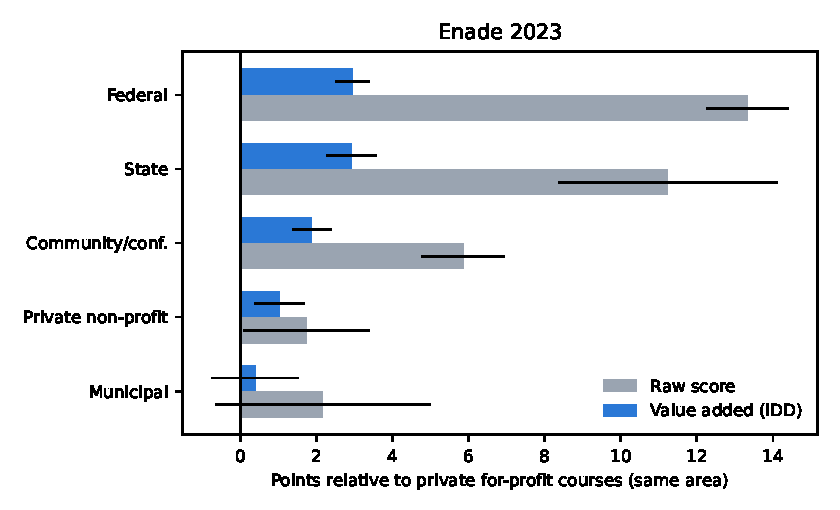
\includegraphics[width=0.75\linewidth]{figures/fig_gaps.pdf}
\caption{Raw score and value-added gaps relative to for-profit private courses of the same area. Coefficients of the regressions with area fixed effects (column 1 of Tables~\ref{tab:regraw} and~\ref{tab:regva}), Enade 2023, with 95\% confidence intervals.}\label{fig:gaps}
\end{figure}

\subsection{Competition for seats}

Table~\ref{tab:selectivity} reports the within-area gaps by level of competition. In the 64 federal courses with fewer than two applicants per seat in 2018, mostly in agronomy, animal science and engineering, the raw gap falls from 12.7 to 7.0 points. The value-added gap falls to 1.4 points, but this result depends on 24 of these courses that reported exactly one applicant per seat, which is more likely a reporting convention than a measure of demand; without them, the raw gap is 9.1 points and the value-added gap 2.6 points, the same as for all federal courses. Above a few applicants per seat, competition matters little: across terciles of applicants per seat within area, the raw gap varies between 12.3 and 13.3 points, and the value-added gap is, if anything, larger in the least competitive tercile.

\begin{table}[!htbp]
\centering\footnotesize
\caption{Federal minus for-profit private courses, by competition for seats in 2018}\label{tab:selectivity}
\resizebox{\linewidth}{!}{\begin{tabular}{lrrcc}
\toprule
Federal courses & Courses & Median applicants/seat & Raw score gap & Value-added gap \\
\midrule
All federal courses & 1{,}465 & 11.6 & 12.7 [12.3, 13.1] & 2.57 [2.33, 2.77] \\
2 or more applicants per seat & 1{,}298 & 12.2 & 12.9 [12.4, 13.3] & 2.59 [2.32, 2.80] \\
Fewer than 2 applicants per seat & 64 & 1.0 & 7.0 [5.5, 8.3] & 1.38 [0.56, 2.04] \\
\quad excluding courses reporting exactly 1.0 & 40 & 1.4 & 9.1 [7.4, 10.8] & 2.56 [1.64, 3.33] \\
Lowest-demand tercile (within area) & 456 & 4.9 & 12.7 [12.0, 13.2] & 3.01 [2.66, 3.30] \\
Middle tercile & 445 & 10.5 & 12.3 [11.6, 12.9] & 2.43 [2.07, 2.75] \\
Highest-demand tercile & 460 & 19.7 & 13.3 [12.5, 14.1] & 2.29 [1.89, 2.68] \\
\bottomrule
\end{tabular}}
\begin{minipage}{\linewidth}\vspace{0.4em}\scriptsize
\textit{Notes:} As in Table~\ref{tab:matched}, Enade 2023. Applicants per seat: applicants divided by new seats in the 2018 Higher Education Census. Terciles are defined within each assessment area. Federal courses without a 2018 Census record are included only in the first row.
\end{minipage}
\end{table}

The regressions in Table~\ref{tab:interactions} confirm this pattern. Competition for seats is positively associated with raw scores in all categories. The federal advantage in raw scores is about 2 to 3 points smaller in low-demand courses, while the federal advantage in value added does not vary with low demand and, measured with the continuous variable, is slightly smaller in the most competitive federal courses. Where federal courses select less, their graduates' advantage at graduation is smaller, but the part of the advantage that the IDD attributes to the course is not.

\begin{table}[!htbp]
\centering\footnotesize
\caption{Interactions between the federal indicator and competition for seats, Enade 2023}\label{tab:interactions}
\resizebox{\linewidth}{!}{\begin{tabular}{lcccc}
\toprule
 & \multicolumn{2}{c}{Raw Enade score} & \multicolumn{2}{c}{Value added (IDD)} \\
\cmidrule(lr){2-3}\cmidrule(lr){4-5}
 & Main & Interaction & Main & Interaction \\
\midrule
log(1 + applicants per seat) $\times$ federal & $1.41^{***}$ (0.28) & $-0.40$ (0.44) & $0.37^{**}$ (0.12) & $-0.49^{*}$ (0.19) \\
Low demand ($<$2) $\times$ federal & $-0.65$ (0.40) & $-2.09^{*}$ (0.91) & $-0.24$ (0.18) & $-0.20$ (0.41) \\
\quad excluding courses reporting exactly 1.0 & $-0.73$ (0.41) & $-3.21^{**}$ (1.01) & $-0.25$ (0.19) & $-0.00$ (0.65) \\
\bottomrule
\end{tabular}}
\begin{minipage}{\linewidth}\vspace{0.4em}\scriptsize
\textit{Notes:} Specification of column 2 of Tables~\ref{tab:regraw} and~\ref{tab:regva} plus the competition variable (``Main'') and its interaction with the federal indicator (``Interaction''). Standard errors clustered by institution in parentheses.
\end{minipage}
\end{table}

\subsection{Robustness}

Table~\ref{tab:robustness} shows that the federal coefficients for 2023 are stable when the regressions are unweighted, when distance-learning courses are excluded, when the sample is restricted to universities, to courses with at least 20 graduates with an Enem score or to courses where at least half of the graduates have an Enem score. Controlling for the course's Enem coverage reduces both coefficients but leaves the share of the raw gap present at entry at 80\%. The value-added gap is also similar in courses with Enem coverage below 50\%, between 50\% and 80\% and above 80\% (2.2, 2.0 and 2.2 points).

\begin{table}[!htbp]
\centering\small
\caption{Robustness of the federal coefficients, Enade 2023}\label{tab:robustness}
\begin{tabular}{lcccr}
\toprule
Specification & Raw score & Value added & Share at entry & Courses \\
\midrule
Baseline (column 2) & 13.20 (0.67) & 2.86 (0.30) & 78\% & 8{,}830 \\
Unweighted & 12.37 (0.66) & 2.59 (0.27) & 79\% & 8{,}830 \\
In-person courses only & 13.59 (0.70) & 2.94 (0.31) & 78\% & 8{,}510 \\
Universities only & 12.63 (0.78) & 2.58 (0.39) & 80\% & 3{,}437 \\
20 or more graduates with an Enem score & 13.14 (0.68) & 2.85 (0.33) & 78\% & 4{,}240 \\
Enem coverage of 50\% or more & 13.50 (0.65) & 2.93 (0.31) & 78\% & 7{,}862 \\
Controlling for Enem coverage & 10.63 (0.57) & 2.13 (0.29) & 80\% & 8{,}830 \\
\bottomrule
\end{tabular}
\begin{minipage}{\linewidth}\vspace{0.4em}\scriptsize
\textit{Notes:} Federal coefficients from the specification of column 2 of Tables~\ref{tab:regraw} and~\ref{tab:regva}. Standard errors clustered by institution in parentheses.
\end{minipage}
\end{table}

\subsection{Earlier editions and the IDD method}\label{sec:method_change}

Table~\ref{tab:series} extends the within-area comparison to every Enade edition with course-level IDD, from 2014 to 2023, using the IDD as published. Each group of areas is assessed every three years, with a four-year gap during the pandemic, so the series contains three editions for each group. For 2014 and 2015 the IDD is taken from the CPC spreadsheets, and the 2015 spreadsheet does not separate for-profit from non-profit private institutions, so the table also reports gaps relative to all private courses. In every edition up to 2021 and in every group of areas, the federal value-added gap lies between $-0.35$ and $0.41$ points, which would put the share of the raw gap present at entry between 95\% and 104\%. In 2022 and 2023, in two different groups of areas, the gap is between 2.0 and 2.7 points. The break coincides with the change in the definition of the IDD described in Section~\ref{sec:background}.

\begin{table}[!htbp]
\centering\small
\caption{Federal minus private courses of the same area, every Enade edition with course-level IDD}\label{tab:series}
\resizebox{\linewidth}{!}{\begin{tabular}{ccrcccc}
\toprule
 & & & \multicolumn{2}{c}{vs.\ private for-profit} & \multicolumn{2}{c}{vs.\ all private} \\
\cmidrule(lr){4-5}\cmidrule(lr){6-7}
Edition & Area group & Federal courses & Raw score & Value added & Raw score & Value added \\
\midrule
2014 & II & 1{,}848 & 8.2 & 0.18 [0.01, 0.39] & 6.0 & $-$0.08 [$-$0.23, 0.05] \\
2015 & III & 567 & -- & -- & 8.0 & $-$0.33 [$-$0.61, $-$0.16] \\
2016 & I & 644 & 8.7 & $-$0.01 [$-$0.11, 0.15] & 8.0 & $-$0.11 [$-$0.22, $-$0.02] \\
2017 & II & 2{,}754 & 8.0 & 0.03 [$-$0.12, 0.31] & 6.4 & $-$0.14 [$-$0.22, $-$0.08] \\
2018 & III & 677 & 10.0 & $-$0.32 [$-$0.43, $-$0.18] & 8.5 & $-$0.35 [$-$0.44, $-$0.27] \\
2019 & I & 1{,}410 & 11.6 & 0.30 [0.23, 0.36] & 10.6 & 0.20 [0.15, 0.26] \\
2021 & II & 2{,}100 & 8.3 & 0.41 [0.29, 0.70] & 7.0 & 0.09 [$-$0.13, 0.19] \\
2022 & III & 731 & 11.7 & 2.70 [2.26, 3.05] & 10.3 & 2.28 [1.91, 2.62] \\
2023 & I & 1{,}465 & 12.7 & 2.57 [2.32, 2.76] & 11.0 & 1.99 [1.76, 2.19] \\
\bottomrule
\end{tabular}}
\begin{minipage}{\linewidth}\vspace{0.4em}\scriptsize
\textit{Notes:} Gaps computed with equation~\eqref{eq:matched}; 95\% bootstrap intervals for the value-added gap in brackets (200 replications). The IDD of 2014 to 2021 was computed with the method in place until 2021; that of 2022 and 2023 with the current method. Area groups follow the three-year Enade cycle: group I (2016, 2019, 2023) covers mainly health and agrarian sciences, group II (2014, 2017, 2021) mainly sciences, humanities and teacher training, and group III (2015, 2018, 2022) mainly applied social sciences such as management and law. Engineering and architecture were assessed in group II until 2017 and in group I from 2019. 2014 and 2015: IDD from the CPC spreadsheets; the 2015 spreadsheet does not distinguish for-profit and non-profit private institutions. There was no Enade in 2020. \textit{Sources:} INEP, Conceito Enade, IDD and CPC spreadsheets, 2014--2023.
\end{minipage}
\end{table}

\begin{figure}[!htbp]
\centering
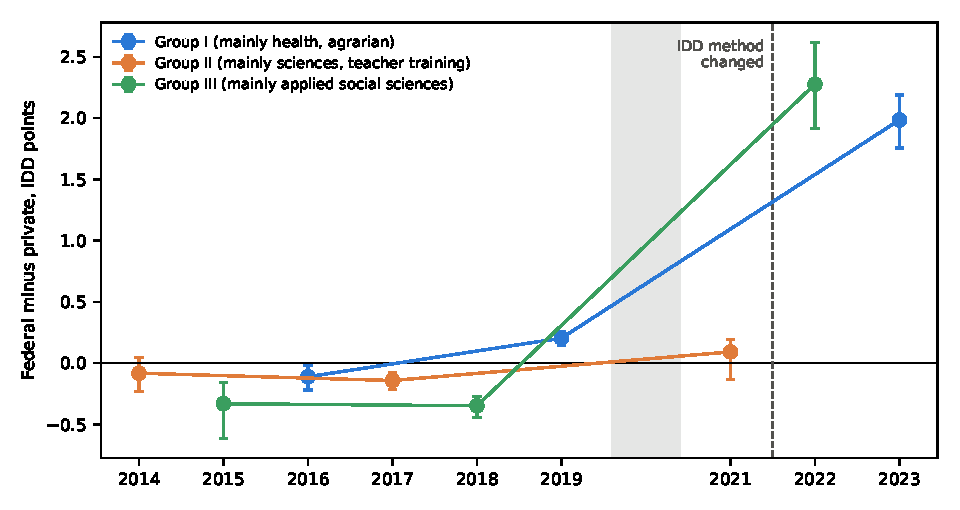
\includegraphics[width=0.8\linewidth]{figures/fig_series.pdf}
\caption{Value-added gap between federal and for-profit private courses of the same area, by Enade edition and group of areas. Solid lines: IDD recomputed with the current method from the student-level microdata, with 95\% bootstrap intervals. Dashed lines: IDD as published. The dotted line marks the change in INEP's method; the shaded band marks the interruption of Enade in 2020.}\label{fig:series}
\end{figure}

In INEP's model, the Enade score of graduate $i$ in course $c$ is $C_{ic}=\gamma_0+u_c+X_{ic}'\beta+e_{ic}$, where $X_{ic}$ are the four Enem scores, $u_c$ is the course's random intercept, with variance $\tau^2$, and $e_{ic}$ has variance $\sigma^2$. Let $\bar r_c$ be the mean of $C_{ic}-\hat\gamma_0-X_{ic}'\hat\beta$ over the $n_c$ graduates of the course with an Enem score. The estimated course effect is the shrunken mean
\begin{equation}\label{eq:blup}
\hat u_c=\lambda_c\,\bar r_c,\qquad \lambda_c=\frac{\tau^2}{\tau^2+\sigma^2/n_c}.
\end{equation}
Until 2021, the predicted score of each graduate included $\hat u_c$, so that, averaged over the graduates used to estimate the model, the raw IDD was the part of the course's mean residual that the model did not attribute to the course \citep{terhaar2021}. From 2022, it is the estimated course effect \citep{inep2023idd}:
\begin{equation}\label{eq:idd}
\mathrm{IDD}^{\mathrm{old}}_c=\bar r_c-\hat u_c=(1-\lambda_c)\,\bar r_c,\qquad \mathrm{IDD}^{\mathrm{new}}_c=\hat u_c=\lambda_c\,\bar r_c .
\end{equation}
As the number of graduates grows, $\lambda_c$ approaches one: the old IDD of a large course approaches zero whatever the course adds, and the new IDD approaches the course's mean residual. In small courses the opposite happens. INEP estimates the model twice and excludes from the second estimation the students whose standardized residual exceeds 3 in absolute value. As shown below, the old IDD was averaged over all graduates, including the excluded ones, so that it also contains their residuals, which are not shrunk.

Table~\ref{tab:method} shows both patterns in the data. With the old method, the dispersion of the raw IDD around the area mean falls from about 5 points in courses with up to five graduates with an Enem score to about 0.4 points in courses with more than 80 in 2019 and 2021, and to 1.1 points or less in every edition from 2014 to 2018. With the new method, it rises with the number of graduates and stabilizes at about 3.2 points. The federal value-added gap follows the same pattern. With the old method, it is 1.6 to 2.1 points among federal courses with fewer than 15 graduates with an Enem score, and about 0.1 points among those with 40 or more, which account for 70\% of federal graduates with an Enem score. With the new method, the gap is largest among the larger courses: 3.6 points in 2022 and 3.3 points in 2023.

\begin{table}[!htbp]
\centering\small
\caption{The IDD method and course size: dispersion of the IDD and federal gaps}\label{tab:method}
\begin{tabular}{lcccc}
\toprule
 & \multicolumn{2}{c}{Method until 2021} & \multicolumn{2}{c}{Method from 2022} \\
\cmidrule(lr){2-3}\cmidrule(lr){4-5}
Graduates with an Enem score in the course & 2019 & 2021 & 2022 & 2023 \\
\midrule
\multicolumn{5}{l}{\textit{A. Standard deviation of the raw IDD around the area mean (points)}} \\
1 to 5 & 4.72 & 4.96 & 1.63 & 2.02 \\
6 to 10 & 2.70 & 2.86 & 2.23 & 2.62 \\
11 to 20 & 1.54 & 1.83 & 2.55 & 3.03 \\
21 to 40 & 0.91 & 1.14 & 2.86 & 3.20 \\
41 to 80 & 0.56 & 0.66 & 3.18 & 3.22 \\
More than 80 & 0.39 & 0.46 & 3.34 & 3.18 \\
\midrule
\multicolumn{5}{l}{\textit{B. Federal minus private for-profit value-added gap (points)}} \\
1 to 14 & 2.10 & 1.61 & 0.35 & 1.15 \\
 & \scriptsize[1.47, 3.50] & \scriptsize[0.48, 2.33] & \scriptsize[$-$0.06, 0.83] & \scriptsize[0.64, 1.74] \\
15 to 39 & 0.53 & 0.51 & 1.26 & 2.54 \\
 & \scriptsize[0.35, 0.73] & \scriptsize[0.26, 0.81] & \scriptsize[0.73, 1.74] & \scriptsize[2.08, 3.03] \\
40 or more & 0.12 & 0.13 & 3.61 & 3.26 \\
 & \scriptsize[0.04, 0.21] & \scriptsize[0.00, 0.32] & \scriptsize[3.01, 4.27] & \scriptsize[2.38, 3.88] \\
All courses & 0.30 & 0.41 & 2.70 & 2.57 \\
 & \scriptsize[0.19, 0.42] & \scriptsize[0.21, 0.71] & \scriptsize[2.07, 3.18] & \scriptsize[2.13, 2.97] \\
\midrule
\multicolumn{5}{l}{\textit{C. Share of the raw gap present at entry (\%)}} \\
1 to 14 & 80 & 66 & 92 & 84 \\
15 to 39 & 95 & 89 & 80 & 77 \\
40 or more & 99 & 99 & 74 & 77 \\
All courses & 97 & 95 & 77 & 80 \\
\bottomrule
\end{tabular}
\begin{minipage}{\linewidth}\vspace{0.4em}\scriptsize
\textit{Notes:} Size bands by the number of participating graduates with a recovered Enem score in the course. Panel A: standard deviation across courses of the raw IDD minus the mean raw IDD of the area. Panels B and C: equation~\eqref{eq:matched} applied to the federal and for-profit courses of each size band; 95\% bootstrap intervals in brackets (200 replications). The 2019 and 2023 editions assessed the same group of areas; 2021 and 2022 assessed groups II and III. \textit{Sources:} INEP, Conceito Enade and IDD spreadsheets; author's calculations.
\end{minipage}
\end{table}

The old method therefore pulls differences between groups of courses toward zero, more so for groups with larger courses. The near-zero federal gaps of 2014 to 2021 are a property of the indicator, not evidence that federal courses added nothing. Where each method distorts least, the two agree with the estimates of Table~\ref{tab:matched}. Among the smallest courses of 2019, where the old method keeps most of the course effect, the federal value-added gap is 2.1 points out of a raw gap of 10.7, so 80\% of the raw gap was present at entry; since part of the course effect is removed even there, this share is an upper bound. Among the courses of 2023 with at least 40 graduates with an Enem score, where the new method shrinks least, the gap is 3.3 points out of 14.2, and 77\% was present at entry. The new method has its own, smaller, bias: it pulls the effects of small courses toward the area mean, which is why the 2022 and 2023 gaps are smaller among them. The shares among courses with 40 or more graduates, 74\% in 2022 and 77\% in 2023, give a sense of the size of this bias for the estimates of Table~\ref{tab:matched}.

These comparisons show that the old method compresses the federal gap; they do not show what the gap would have been under the current method. To answer that, I recomputed the IDD from INEP's student-level microdata \citep{inepiddmicro}. For each area and edition, I estimated the model by restricted maximum likelihood, excluded the students with an absolute standardized residual above 3, estimated it again, and computed the IDD with both definitions. The computation reproduces the published values: the correlation between the published raw IDD and the recomputed one is 1.00 in every edition from 2016 to 2023, with the old definition up to 2021 and the current one from 2022, and the median absolute difference is below 0.01 points. The old definition is reproduced only when the mean residual is taken over all graduates, including those excluded as outliers. The editions of 2014 and 2015 are not recomputed because their published spreadsheets have no course codes to link with.

\begin{table}[!htbp]
\centering\small
\caption{Federal minus private courses of the same area, with the IDD recomputed from student-level data}\label{tab:recomputed}
\resizebox{\linewidth}{!}{\begin{tabular}{cccccc}
\toprule
 & & & \multicolumn{2}{c}{Value-added gap} & Share of raw gap \\
\cmidrule(lr){4-5}
Edition & Area group & Raw score gap & Published IDD & Current method & present at entry \\
\midrule
\multicolumn{6}{l}{\textit{A. Relative to private for-profit courses}} \\
2016 & I & 8.7 & $-$0.01 & 0.75 [0.12, 1.35] & 91\% \\
2017 & II & 8.0 & 0.03 & 1.38 [0.75, 1.92] & 83\% \\
2018 & III & 10.0 & $-$0.32 & 0.87 [0.20, 1.45] & 91\% \\
2019 & I & 11.6 & 0.30 & 1.85 [1.42, 2.25] & 84\% \\
2021 & II & 8.3 & 0.41 & 2.36 [1.64, 2.92] & 71\% \\
2022 & III & 11.7 & 2.70 & 2.70 [2.09, 3.22] & 77\% \\
2023 & I & 12.7 & 2.57 & 2.57 [2.13, 2.93] & 80\% \\
\midrule
\multicolumn{6}{l}{\textit{B. Relative to all private courses}} \\
2016 & I & 8.0 & $-$0.11 & 0.51 [$-$0.03, 0.99] & 94\% \\
2017 & II & 6.4 & $-$0.14 & 0.79 [0.30, 1.16] & 88\% \\
2018 & III & 8.5 & $-$0.35 & 0.58 [0.01, 1.17] & 93\% \\
2019 & I & 10.6 & 0.20 & 1.51 [1.07, 1.88] & 86\% \\
2021 & II & 7.0 & 0.09 & 1.79 [1.00, 2.30] & 74\% \\
2022 & III & 10.3 & 2.28 & 2.28 [1.70, 2.80] & 78\% \\
2023 & I & 11.0 & 1.99 & 1.99 [1.45, 2.39] & 82\% \\
\bottomrule
\end{tabular}}
\begin{minipage}{\linewidth}\vspace{0.4em}\scriptsize
\textit{Notes:} Gaps computed with equation~\eqref{eq:matched}. ``Published IDD'': raw IDD published by INEP (old definition up to 2021, current definition from 2022). ``Current method'': raw IDD recomputed with the current definition (the estimated course intercept) from the IDD microdata; for 2022 and 2023 it coincides with the published value. 95\% bootstrap intervals in brackets (200 replications). The share of the raw gap present at entry uses the current method. \textit{Sources:} INEP, IDD microdata and Conceito Enade and IDD spreadsheets, 2016--2023; author's calculations.
\end{minipage}
\end{table}

Table~\ref{tab:recomputed} and Figure~\ref{fig:series} report the result. With a consistent definition, the federal value-added advantage over for-profit courses is positive in every edition: 0.75, 1.38 and 0.87 points in 2016, 2017 and 2018, 1.85 points in 2019, 2.36 points in 2021, and 2.70 and 2.57 points in 2022 and 2023. The old method therefore hid most of the federal advantage. The advantage also grew: within each group of areas, from 0.75 to 1.85 and 2.57 points in group I, from 1.38 to 2.36 points in group II and from 0.87 to 2.70 points in group III, with confidence intervals that do not overlap between the first and the last edition of each group. The jump in the published series thus combines a change of method with a real increase. Even so, the share of the raw gap present at entry stays between 71\% and 91\% in every edition. This paper does not examine why the advantage grew; possible reasons include the expansion of distance learning in for-profit institutions, changes in which graduates have a recovered Enem score, and changes in the composition of federal entrants after the quota law.

\subsection{Cost and value added among federal universities}

Among the 66 federal universities with sufficient data, current cost per in-person undergraduate in 2024 ranged from about R\$~21,000 to R\$~55,000, with a median of R\$~40,000. Figure~\ref{fig:cost} and Table~\ref{tab:cost} show that higher spending is not associated with more value added. The third of universities with the highest cost spend on average R\$~48,000 per student, R\$~9,000 more than the middle third, and have a lower mean value added (1.5 against 1.9 points). The slope of value added on cost is 0.03 points per R\$~1,000, with a correlation of 0.17 that is not statistically significant. Graduate-program intensity explains about a third of the variation in cost across universities (graduate students per undergraduate and the mean CAPES grade together have an $R^2$ of 0.35), but controlling for it leaves the slope of value added on cost unchanged (0.03, $t=1.1$).

\begin{table}[!htbp]
\centering\small
\caption{Cost per student and value added, federal universities}\label{tab:cost}
\begin{tabular}{lccc}
\toprule
Cost tercile & Universities & Cost per student (R\$ thousand) & Value added (IDD) \\
\midrule
Lowest & 22 & 29.7 & 0.70 \\
Middle & 22 & 39.2 & 1.94 \\
Highest & 22 & 48.0 & 1.48 \\
\bottomrule
\end{tabular}
\begin{minipage}{\linewidth}\vspace{0.4em}\scriptsize
\textit{Notes:} 66 federal universities with at least 30 graduates with an Enem score in Enade 2023; UNIVASF excluded because of inconsistent enrolment data. Cost: current spending in 2024 excluding pensions, special charges, capital and university hospitals, divided by in-person undergraduate enrolments in 2024. Value added: mean raw IDD of the university's courses relative to the area mean, weighted by graduates with an Enem score. \textit{Sources:} Portal da Transpar\^encia; 2024 Higher Education Census; INEP, IDD 2023.
\end{minipage}
\end{table}

\begin{figure}[!htbp]
\centering
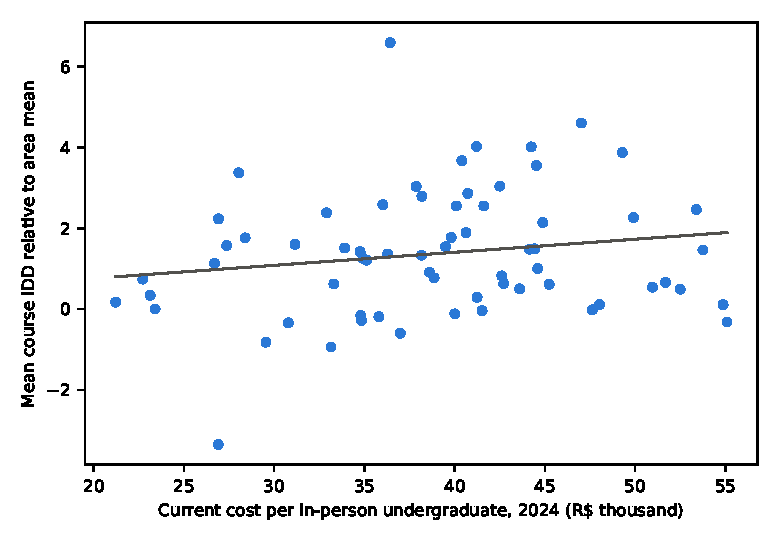
\includegraphics[width=0.72\linewidth]{figures/fig_cost.pdf}
\caption{Current cost per in-person undergraduate (2024) and mean value added (IDD 2023), 66 federal universities, with the least-squares line.}\label{fig:cost}
\end{figure}

%======================================================================
\section{Discussion}\label{sec:discussion}
%======================================================================

The main result holds across specifications, samples and the two editions computed with the current method: about four fifths of the advantage of federal graduates at graduation was present at entry. What remains is a value-added advantage of about a fifth of a student standard deviation in 2022 and 2023, larger than in earlier editions once they are computed with the same method. That federal universities spend considerably more per student than private institutions, and that spending more does not predict more value added across federal universities, suggests that the additional cost buys little additional learning as measured by Enade.

Several limitations qualify these conclusions. The IDD only controls for what the Enem measures; unobserved differences in motivation, effort or study conditions between federal and private students, such as the time available for study during the course, would bias the value-added gap, most likely in favour of the more selective federal courses, which would strengthen the conclusion that the gap is mostly selection. The model behind the IDD also assumes that course effects are unrelated to students' Enem scores; if better courses attract students with higher scores, the Enem coefficients absorb part of the course effect and the IDD understates the value added of selective courses. The current IDD shrinks the effects of small courses, as shown in Section~\ref{sec:method_change}. The recomputation of the earlier editions shows that the federal advantage grew between 2016 and 2023, but the reasons for this growth are not examined here. The IDD is computed only for graduates with a recovered Enem score, whose share differs across categories and editions. Enade measures learning in a single exam that has no consequences for students, and differences in effort across institutions cannot be ruled out. The analysis is at the course level because public microdata do not link individual scores to individual characteristics; access to identified data through INEP's protected-data service would allow student-level estimates with richer controls. Finally, the analysis compares the federal sector with the for-profit private sector, which serves a different population and charges tuition; a comparison of costs between the two sectors depends on how research, pensions and the tuition paid in the private sector are treated \citep{bielschowsky2022}.

The comparison with private institutions also bears on a policy that already exists. Through ProUni, private institutions receive tax exemptions in exchange for tuition-free places for low-income students, who are admitted on their Enem scores. \citet{almeida2022} put the program's tax expenditure at about R\$~13.5 billion between 2005 and 2017, at 2020 prices, for 2.2 million scholarship-years, or about R\$~6,000 per scholarship-year. In the Enade editions from 2012 to 2014, ProUni scholarship holders scored above their classmates in the same course and institution \citep{wainer2018}. These results do not show that ProUni students learn as much as they would in a federal university: the comparison is with classmates, not with federal students, scholarship holders are selected on their Enem scores, and the tax expenditure is not the full cost of their education. Together with the small value-added gap documented here, they suggest that the cost of a place in a federal university should be compared with that of alternatives such as ProUni, and not only with the tuition of a private course.

%======================================================================
\section{Conclusion}\label{sec:conclusion}
%======================================================================

Federal universities in Brazil graduate students who score far above those of for-profit private institutions, but most of that advantage was there when the students arrived. Between 71\% and 91\% of the raw gap in the national graduation exam corresponds to differences at entry, in every edition from 2016 to 2023 computed with the current value-added method; where federal courses select less, their raw advantage shrinks by about half. The value-added advantage that remains grew from about 1 point to 2.6--2.7 points on a 0--100 scale, about a fifth of a student standard deviation in the most recent editions. The official indicator hid it until 2021, because the method then in use removed most of each course's own effect, the more so the larger the course. Within the federal system, spending more per student is not associated with more value added. Raw indicators of quality, which reward selection, are therefore a poor guide to how much public universities teach.

\section*{Data and code availability}
All data are public. Code and intermediate results are available at \url{https://github.com/Caioalexnes/higher-education-analysis}; a versioned copy will be deposited on Zenodo.

\section*{Declaration of generative AI use}
The analysis code, tables, figures and a first draft of this text were produced with the assistance of a generative AI system (Claude, Anthropic), working under the author's direction. The author reviewed the code, the results and the text, and takes full responsibility for the content, including the accuracy of the references.

\section*{Funding and competing interests}
The author received no funding for this work and reports no competing interests.

\bibliographystyle{plainnat}
\bibliography{refs}

\end{document}
